% Options for packages loaded elsewhere
\PassOptionsToPackage{unicode}{hyperref}
\PassOptionsToPackage{hyphens}{url}
\PassOptionsToPackage{dvipsnames,svgnames,x11names}{xcolor}
%
\documentclass[
  a4paper,
]{ctexart}

\usepackage{amsmath,amssymb}
\usepackage{iftex}
\ifPDFTeX
  \usepackage[T1]{fontenc}
  \usepackage[utf8]{inputenc}
  \usepackage{textcomp} % provide euro and other symbols
\else % if luatex or xetex
  \usepackage{unicode-math}
  \defaultfontfeatures{Scale=MatchLowercase}
  \defaultfontfeatures[\rmfamily]{Ligatures=TeX,Scale=1}
\fi
\usepackage{lmodern}
\ifPDFTeX\else  
    % xetex/luatex font selection
\fi
% Use upquote if available, for straight quotes in verbatim environments
\IfFileExists{upquote.sty}{\usepackage{upquote}}{}
\IfFileExists{microtype.sty}{% use microtype if available
  \usepackage[]{microtype}
  \UseMicrotypeSet[protrusion]{basicmath} % disable protrusion for tt fonts
}{}
\makeatletter
\@ifundefined{KOMAClassName}{% if non-KOMA class
  \IfFileExists{parskip.sty}{%
    \usepackage{parskip}
  }{% else
    \setlength{\parindent}{0pt}
    \setlength{\parskip}{6pt plus 2pt minus 1pt}}
}{% if KOMA class
  \KOMAoptions{parskip=half}}
\makeatother
\usepackage{xcolor}
\setlength{\emergencystretch}{3em} % prevent overfull lines
\setcounter{secnumdepth}{5}
% Make \paragraph and \subparagraph free-standing
\ifx\paragraph\undefined\else
  \let\oldparagraph\paragraph
  \renewcommand{\paragraph}[1]{\oldparagraph{#1}\mbox{}}
\fi
\ifx\subparagraph\undefined\else
  \let\oldsubparagraph\subparagraph
  \renewcommand{\subparagraph}[1]{\oldsubparagraph{#1}\mbox{}}
\fi


\providecommand{\tightlist}{%
  \setlength{\itemsep}{0pt}\setlength{\parskip}{0pt}}\usepackage{longtable,booktabs,array}
\usepackage{calc} % for calculating minipage widths
% Correct order of tables after \paragraph or \subparagraph
\usepackage{etoolbox}
\makeatletter
\patchcmd\longtable{\par}{\if@noskipsec\mbox{}\fi\par}{}{}
\makeatother
% Allow footnotes in longtable head/foot
\IfFileExists{footnotehyper.sty}{\usepackage{footnotehyper}}{\usepackage{footnote}}
\makesavenoteenv{longtable}
\usepackage{graphicx}
\makeatletter
\def\maxwidth{\ifdim\Gin@nat@width>\linewidth\linewidth\else\Gin@nat@width\fi}
\def\maxheight{\ifdim\Gin@nat@height>\textheight\textheight\else\Gin@nat@height\fi}
\makeatother
% Scale images if necessary, so that they will not overflow the page
% margins by default, and it is still possible to overwrite the defaults
% using explicit options in \includegraphics[width, height, ...]{}
\setkeys{Gin}{width=\maxwidth,height=\maxheight,keepaspectratio}
% Set default figure placement to htbp
\makeatletter
\def\fps@figure{htbp}
\makeatother
\newlength{\cslhangindent}
\setlength{\cslhangindent}{1.5em}
\newlength{\csllabelwidth}
\setlength{\csllabelwidth}{3em}
\newlength{\cslentryspacingunit} % times entry-spacing
\setlength{\cslentryspacingunit}{\parskip}
\newenvironment{CSLReferences}[2] % #1 hanging-ident, #2 entry spacing
 {% don't indent paragraphs
  \setlength{\parindent}{0pt}
  % turn on hanging indent if param 1 is 1
  \ifodd #1
  \let\oldpar\par
  \def\par{\hangindent=\cslhangindent\oldpar}
  \fi
  % set entry spacing
  \setlength{\parskip}{#2\cslentryspacingunit}
 }%
 {}
\usepackage{calc}
\newcommand{\CSLBlock}[1]{#1\hfill\break}
\newcommand{\CSLLeftMargin}[1]{\parbox[t]{\csllabelwidth}{#1}}
\newcommand{\CSLRightInline}[1]{\parbox[t]{\linewidth - \csllabelwidth}{#1}\break}
\newcommand{\CSLIndent}[1]{\hspace{\cslhangindent}#1}

\makeatletter
\makeatother
\makeatletter
\@ifpackageloaded{bookmark}{}{\usepackage{bookmark}}
\makeatother
\makeatletter
\@ifpackageloaded{caption}{}{\usepackage{caption}}
\AtBeginDocument{%
\ifdefined\contentsname
  \renewcommand*\contentsname{Table of contents}
\else
  \newcommand\contentsname{Table of contents}
\fi
\ifdefined\listfigurename
  \renewcommand*\listfigurename{List of Figures}
\else
  \newcommand\listfigurename{List of Figures}
\fi
\ifdefined\listtablename
  \renewcommand*\listtablename{List of Tables}
\else
  \newcommand\listtablename{List of Tables}
\fi
\ifdefined\figurename
  \renewcommand*\figurename{Figure}
\else
  \newcommand\figurename{Figure}
\fi
\ifdefined\tablename
  \renewcommand*\tablename{Table}
\else
  \newcommand\tablename{Table}
\fi
}
\@ifpackageloaded{float}{}{\usepackage{float}}
\floatstyle{ruled}
\@ifundefined{c@chapter}{\newfloat{codelisting}{h}{lop}}{\newfloat{codelisting}{h}{lop}[chapter]}
\floatname{codelisting}{Listing}
\newcommand*\listoflistings{\listof{codelisting}{List of Listings}}
\makeatother
\makeatletter
\@ifpackageloaded{caption}{}{\usepackage{caption}}
\@ifpackageloaded{subcaption}{}{\usepackage{subcaption}}
\makeatother
\makeatletter
\@ifpackageloaded{tcolorbox}{}{\usepackage[skins,breakable]{tcolorbox}}
\makeatother
\makeatletter
\@ifundefined{shadecolor}{\definecolor{shadecolor}{rgb}{.97, .97, .97}}
\makeatother
\makeatletter
\makeatother
\makeatletter
\makeatother
\ifLuaTeX
  \usepackage{selnolig}  % disable illegal ligatures
\fi
\IfFileExists{bookmark.sty}{\usepackage{bookmark}}{\usepackage{hyperref}}
\IfFileExists{xurl.sty}{\usepackage{xurl}}{} % add URL line breaks if available
\urlstyle{same} % disable monospaced font for URLs
\hypersetup{
  pdftitle={Adrian Dairy Traveling},
  pdfauthor={Norah Jones},
  colorlinks=true,
  linkcolor={blue},
  filecolor={Maroon},
  citecolor={Blue},
  urlcolor={Blue},
  pdfcreator={LaTeX via pandoc}}

\title{Adrian Dairy Traveling}
\author{Norah Jones}
\date{2023-06-22}

\begin{document}
\maketitle
\ifdefined\Shaded\renewenvironment{Shaded}{\begin{tcolorbox}[frame hidden, boxrule=0pt, borderline west={3pt}{0pt}{shadecolor}, breakable, enhanced, interior hidden, sharp corners]}{\end{tcolorbox}}\fi

\renewcommand*\contentsname{Table of contents}
{
\hypersetup{linkcolor=}
\setcounter{tocdepth}{2}
\tableofcontents
}
\bookmarksetup{startatroot}

\hypertarget{preface}{%
\chapter*{Preface}\label{preface}}
\addcontentsline{toc}{chapter}{Preface}

\markboth{Preface}{Preface}

\begin{quote}
``他在田野上遊蕩,狼吞虎嚥著所看到的四處的一切。''
\end{quote}

\begin{quote}
《禪與摩托車維修的藝術》
\end{quote}

玫瑰說,疫情前的地球對她來說像個水球一樣,真的是踩下去會彈起來的狀態;但疫情後地球就乾涸了,充滿了Barrier(玫瑰
2023)。

深以為然。

與其說怪疫情,不如直面我們生活的時代:一個走向封閉的時代。

我們``忠誠、呼籲'',希望大人們迷途知返,但回頭來,只能承認我們是``沒有用的年輕人''(好樂團
GoodBand 2022),於是我們選擇``退出''。(Hirschman 2004)
拾起那把本該屬於我們的廉航包,保持憤怒地、快樂的擁抱我們自己的世界。

疫情三年,漫長又快速。

我們在``層層加碼''的封控政策和``政治抑鬱''中掙扎,
但回憶時卻幾乎完全不剩下什麼。
封控政策在一朝一夕間快速結束,但很多事情悄然間讓國人習以為然:對強大政府的依賴、對封鎖的合理化、對外界的近乎自然的排斥。

2023年4月,在經歷了3年的疫情封鎖後,我在``後疫情''第一次出走。
如果說Penang的海是為了一場不那麼容易的告別,那當我收拾行李飛往ChiangMai的時候,我想我已經準備好了一段只屬於我自己的旅程。

走出去,和過去的人告別:

開始的時候是為了向別人證明,我不是你刻板印象中的那樣,但自己也那不準,我是不是真的就是那樣?
後來卻發現,我真的不能被任何人定義。別TM告訴我我是哪樣。

走出去,和``祖國''告別:

還沒放下憤怒,但至少變得冷漠。

走出去,``在田野上遊蕩,狼吞虎嚥著所看到的四處的一切。'' (Pirsig 1974)

\bookmarksetup{startatroot}

\hypertarget{malaysia-ux539fux4f86ux4ed6ux5011ux751fux6d3bux7684ux9019ux9ebcux81eaux7531}{%
\chapter{Malaysia:
原來他們生活的這麼自由}\label{malaysia-ux539fux4f86ux4ed6ux5011ux751fux6d3bux7684ux9019ux9ebcux81eaux7531}}

\bookmarksetup{startatroot}

\hypertarget{thailand-ux8981ux4ec0ux9ebcux570bux5bb6ux80fdux529b}{%
\chapter{Thailand:
要什麼國家能力!}\label{thailand-ux8981ux4ec0ux9ebcux570bux5bb6ux80fdux529b}}

\bookmarksetup{startatroot}

\hypertarget{vietnam-ux897fux8ca2ux4e03ux65e5}{%
\chapter{Vietnam: 西貢七日}\label{vietnam-ux897fux8ca2ux4e03ux65e5}}

西貢作為南越舊都,在很多電影和文章裡都是以風情萬種的形象出現,民國112年6月,我借徑泰國
\textbf{?@sec-thailand} 從ChiangMai出發,在胡志明市度過了7天的時間。

\hypertarget{ux7e3dux9ad4ux5370ux8c61}{%
\section{總體印象}\label{ux7e3dux9ad4ux5370ux8c61}}

\textbf{?@fig-summary}

其實我對西貢的總體印象是如 \textbf{?@fig-summary} 所示。
來西貢之前,這是一個被國內很多人認為是同上世紀上海相似的地方(也的確有這些感官)。
在中國國內的社群媒體和YouTube平台上基本都是用''男人天堂''、``飛車搶匪''、``按摩洗頭''等詞彙來描述西貢。
初到這個城市的時候,這裡對我來說是以革命領袖胡志明名字命名的越南社會主義民主共和國的一個大城市。
雖然多以機車🛵代步,但駕駛習慣和泰國截然不同,就像本地人常用的叫車軟體''Be''一樣,一下飛機就能充斥到''Beeeeee''的喇叭聲,充斥了7天。可以說在西貢的前兩天,我每天都在看去其他地方的機票,甚至有想買票回ChiangMai。
改變我對胡志明市印象的是它的街角和民眾。在街角喝咖啡的時候,胡志明市悄悄然的就變成了西貢。
西貢的七日,也經歷了無數被當地朋友''Make my day''的時刻。
坦誠的講,在來到越南尤其是胡志明市在小紅書上的形象大多是負面的,政府腐敗、民眾狡猾、社會落後、治安混亂。
西貢七日,再次讓我質疑中國社群媒體的''透鏡效應'',不知是中國人本身在越南的名聲不好,還是民眾的大國感,我感受到的西貢是一個比國內開放、包容的多的城市。
與我來說,它並不是一個很適合Chill的地方,但卻有很多值得享受和思考的地方。

\begin{figure}

{\centering \includegraphics{Vietnam_files/figure-pdf/fig-summary-1.pdf}

}

\caption{\label{fig-summary-1}對西貢的總體印象}

\end{figure}

\begin{figure}

{\centering \includegraphics{Vietnam_files/figure-pdf/fig-summary-2.pdf}

}

\caption{\label{fig-summary-2}對西貢的總體印象}

\end{figure}

\hypertarget{day1}{%
\section{Day1}\label{day1}}

我是民國112年6月15日下午從清邁國際機場乘坐越南廉價航空公司''越捷航空''出發的。
一個蠻有趣的細節是在清邁機場書店中看到有關中國的一本書''China in ten
words'',這可能是泰國民眾在來中國之前對中國的初印象(
Figure~\ref{fig-CNin10words} )。
不得不感嘆時間和形式的變化,``人民''、``領袖''、``革命''、``差距''在中國社會變得更加重要,其他的詞彙似乎已不適合描述當下的中國。

不知道越南的社會主義建設的如何呢?

\begin{figure}

{\centering \includegraphics{figures/fig-CNin10words.png}

}

\caption{\label{fig-CNin10words}China in ten words}

\end{figure}

在飛機上的鄰座是一個在胡志明市生活的小姐,她的描述給了我對西貢的第一印象,比清邁''貴得多''。當我借助翻譯軟體問她覺得胡志明市社會主義的氛圍怎麼樣,她非常肯定的笑著跟我說''沒多少''。

\begin{figure}

{\centering \includegraphics{figures/VietjetFlight.png}

}

\caption{越捷航空航班}

\end{figure}

持中國護照到越南可以在提前通過淘寶購買批文後,在機場申請Landing Visa。
有趣的一點是,由於中越兩國在南中國海(越南稱東海)領土主權上的爭議,以及中國新版護照(E開頭)24頁等處印有完整版的中國地圖(也是服,明知道有爭議,就不能替出行民眾想下麼\ldots.越南政府也是有夠小肚雞腸的)。
因此在官方意義上,越南政府並不承認中國的新版護照,因此中國民眾無法申請貼紙簽,而是獲批一張單獨的簽證紙,謂之貼紙簽。
兩個社會主義BuddyBuddy之前的兄弟情義可見一斑啊。

\bookmarksetup{startatroot}

\hypertarget{uae-ux71b1}{%
\chapter{UAE: 熱}\label{uae-ux71b1}}

\bookmarksetup{startatroot}

\hypertarget{netherlands-a-safe-place-for-diversity}{%
\chapter{Netherlands: A safe place for
diversity}\label{netherlands-a-safe-place-for-diversity}}

\bookmarksetup{startatroot}

\hypertarget{belgium-not-that-poor-but-so-sexy}{%
\chapter{Belgium: Not that poor but so
SEXY}\label{belgium-not-that-poor-but-so-sexy}}

\bookmarksetup{startatroot}

\hypertarget{ux897fux8ca2ux4e03ux65e5}{%
\chapter{西貢七日}\label{ux897fux8ca2ux4e03ux65e5}}

西貢作為南越舊都,在很多電影和文章裡都是以風情萬種的形象出現,民國112年6月,我借徑泰國
\textbf{?@sec-thailand} 從ChiangMai出發,在胡志明市度過了7天的時間。

\hypertarget{ux7e3dux9ad4ux5370ux8c61-1}{%
\section{總體印象}\label{ux7e3dux9ad4ux5370ux8c61-1}}

\textbf{?@fig-summary}

其實我對西貢的總體印象是如 \textbf{?@fig-summary} 所示。
來西貢之前,這是一個被國內很多人認為是同上世紀上海相似的地方(也的確有這些感官)。
在中國國內的社群媒體和YouTube平台上基本都是用''男人天堂''、``飛車搶匪''、``按摩洗頭''等詞彙來描述西貢。
初到這個城市的時候,這裡對我來說是以革命領袖胡志明名字命名的越南社會主義民主共和國的一個大城市。
雖然多以機車🛵代步,但駕駛習慣和泰國截然不同,就像本地人常用的叫車軟體''Be''一樣,一下飛機就能充斥到''Beeeeee''的喇叭聲,充斥了7天。可以說在西貢的前兩天,我每天都在看去其他地方的機票,甚至有想買票回ChiangMai。
改變我對胡志明市印象的是它的街角和民眾。在街角喝咖啡的時候,胡志明市悄悄然的就變成了西貢。
西貢的七日,也經歷了無數被當地朋友''Make my day''的時刻。
坦誠的講,在來到越南尤其是胡志明市在小紅書上的形象大多是負面的,政府腐敗、民眾狡猾、社會落後、治安混亂。
西貢七日,再次讓我質疑中國社群媒體的''透鏡效應'',不知是中國人本身在越南的名聲不好,還是民眾的大國感,我感受到的西貢是一個比國內開放、包容的多的城市。
與我來說,它並不是一個很適合Chill的地方,但卻有很多值得享受和思考的地方。

\begin{figure}

{\centering \includegraphics{Japan_files/figure-pdf/fig-summary-1.pdf}

}

\caption{\label{fig-summary-1}對西貢的總體印象}

\end{figure}

\begin{figure}

{\centering \includegraphics{Japan_files/figure-pdf/fig-summary-2.pdf}

}

\caption{\label{fig-summary-2}對西貢的總體印象}

\end{figure}

\hypertarget{day1-1}{%
\section{Day1}\label{day1-1}}

我是民國112年6月15日下午從清邁國際機場乘坐越南廉價航空公司''越捷航空''出發的。
一個蠻有趣的細節是在清邁機場書店中看到有關中國的一本書''China in ten
words'',這可能是泰國民眾在來中國之前對中國的初印象(
Figure~\ref{fig-CNin10words} )。
不得不感嘆時間和形式的變化,``人民''、``領袖''、``革命''、``差距''在中國社會變得更加重要,其他的詞彙似乎已不適合描述當下的中國。

不知道越南的社會主義建設的如何呢?

\begin{figure}

{\centering \includegraphics{figures/fig-CNin10words.png}

}

\caption{\label{fig-CNin10words}China in ten words}

\end{figure}

在飛機上的鄰座是一個在胡志明市生活的小姐,她的描述給了我對西貢的第一印象,比清邁''貴得多''。當我借助翻譯軟體問她覺得胡志明市社會主義的氛圍怎麼樣,她非常肯定的笑著跟我說''沒多少''。

\begin{figure}

{\centering \includegraphics{figures/VietjetFlight.png}

}

\caption{越捷航空航班}

\end{figure}

持中國護照到越南可以在提前通過淘寶購買批文後,在機場申請Landing Visa。
有趣的一點是,由於中越兩國在南中國海(越南稱東海)領土主權上的爭議,以及中國新版護照(E開頭)24頁等處印有完整版的中國地圖(也是服,明知道有爭議,就不能替出行民眾想下麼\ldots.越南政府也是有夠小肚雞腸的)。
因此在官方意義上,越南政府並不承認中國的新版護照,因此中國民眾無法申請貼紙簽,而是獲批一張單獨的簽證紙,謂之貼紙簽。
兩個社會主義BuddyBuddy之前的兄弟情義可見一斑啊。

\bookmarksetup{startatroot}

\hypertarget{ux897fux8ca2ux4e03ux65e5-1}{%
\chapter{西貢七日}\label{ux897fux8ca2ux4e03ux65e5-1}}

西貢作為南越舊都,在很多電影和文章裡都是以風情萬種的形象出現,民國112年6月,我借徑泰國
\textbf{?@sec-thailand} 從ChiangMai出發,在胡志明市度過了7天的時間。

\hypertarget{ux7e3dux9ad4ux5370ux8c61-2}{%
\section{總體印象}\label{ux7e3dux9ad4ux5370ux8c61-2}}

\textbf{?@fig-summary}

其實我對西貢的總體印象是如 \textbf{?@fig-summary} 所示。
來西貢之前,這是一個被國內很多人認為是同上世紀上海相似的地方(也的確有這些感官)。
在中國國內的社群媒體和YouTube平台上基本都是用''男人天堂''、``飛車搶匪''、``按摩洗頭''等詞彙來描述西貢。
初到這個城市的時候,這裡對我來說是以革命領袖胡志明名字命名的越南社會主義民主共和國的一個大城市。
雖然多以機車🛵代步,但駕駛習慣和泰國截然不同,就像本地人常用的叫車軟體''Be''一樣,一下飛機就能充斥到''Beeeeee''的喇叭聲,充斥了7天。可以說在西貢的前兩天,我每天都在看去其他地方的機票,甚至有想買票回ChiangMai。
改變我對胡志明市印象的是它的街角和民眾。在街角喝咖啡的時候,胡志明市悄悄然的就變成了西貢。
西貢的七日,也經歷了無數被當地朋友''Make my day''的時刻。
坦誠的講,在來到越南尤其是胡志明市在小紅書上的形象大多是負面的,政府腐敗、民眾狡猾、社會落後、治安混亂。
西貢七日,再次讓我質疑中國社群媒體的''透鏡效應'',不知是中國人本身在越南的名聲不好,還是民眾的大國感,我感受到的西貢是一個比國內開放、包容的多的城市。
與我來說,它並不是一個很適合Chill的地方,但卻有很多值得享受和思考的地方。

\begin{figure}

{\centering \includegraphics{Korea_files/figure-pdf/fig-summary-1.pdf}

}

\caption{\label{fig-summary-1}對西貢的總體印象}

\end{figure}

\begin{figure}

{\centering \includegraphics{Korea_files/figure-pdf/fig-summary-2.pdf}

}

\caption{\label{fig-summary-2}對西貢的總體印象}

\end{figure}

\hypertarget{day1-2}{%
\section{Day1}\label{day1-2}}

我是民國112年6月15日下午從清邁國際機場乘坐越南廉價航空公司''越捷航空''出發的。
一個蠻有趣的細節是在清邁機場書店中看到有關中國的一本書''China in ten
words'',這可能是泰國民眾在來中國之前對中國的初印象(
Figure~\ref{fig-CNin10words} )。
不得不感嘆時間和形式的變化,``人民''、``領袖''、``革命''、``差距''在中國社會變得更加重要,其他的詞彙似乎已不適合描述當下的中國。

不知道越南的社會主義建設的如何呢?

\begin{figure}

{\centering \includegraphics{figures/fig-CNin10words.png}

}

\caption{\label{fig-CNin10words}China in ten words}

\end{figure}

在飛機上的鄰座是一個在胡志明市生活的小姐,她的描述給了我對西貢的第一印象,比清邁''貴得多''。當我借助翻譯軟體問她覺得胡志明市社會主義的氛圍怎麼樣,她非常肯定的笑著跟我說''沒多少''。

\begin{figure}

{\centering \includegraphics{figures/VietjetFlight.png}

}

\caption{越捷航空航班}

\end{figure}

持中國護照到越南可以在提前通過淘寶購買批文後,在機場申請Landing Visa。
有趣的一點是,由於中越兩國在南中國海(越南稱東海)領土主權上的爭議,以及中國新版護照(E開頭)24頁等處印有完整版的中國地圖(也是服,明知道有爭議,就不能替出行民眾想下麼\ldots.越南政府也是有夠小肚雞腸的)。
因此在官方意義上,越南政府並不承認中國的新版護照,因此中國民眾無法申請貼紙簽,而是獲批一張單獨的簽證紙,謂之貼紙簽。
兩個社會主義BuddyBuddy之前的兄弟情義可見一斑啊。

\bookmarksetup{startatroot}

\hypertarget{references}{%
\chapter*{References}\label{references}}
\addcontentsline{toc}{chapter}{References}

\markboth{References}{References}

\hypertarget{refs}{}
\begin{CSLReferences}{1}{0}
\leavevmode\vadjust pre{\hypertarget{ref-Hirschman2004a}{}}%
Hirschman, Albert O. 2004. \emph{Exit, Voice, and Loyalty: Responses to
Decline in Firms, Organizations, and States}. {Cambridge, Mass}:
{Harvard University Press}.

\leavevmode\vadjust pre{\hypertarget{ref-Pirsig1974}{}}%
Pirsig, Robert M. 1974. \emph{Zen and the Art of Motorcycle Maintenance:
An Inquiry into Values}. {New York}: {Morrow}.

\leavevmode\vadjust pre{\hypertarget{ref-HaoLeTuanGoodBand2022}{}}%
好樂團 GoodBand, dir. 2022. \emph{好樂團 {GoodBand} ---
他們說我是沒有用的年輕人 {Official Music Video}}.
\url{https://www.youtube.com/watch?v=LH8n44-ocLk}.

\leavevmode\vadjust pre{\hypertarget{ref-MeiGui2023}{}}%
玫瑰. 2023.
{``玫瑰:城市的大街不应该只是你玩命赶路的地方,大街就是乐子本身.''}
{Подкасти Apple}. 2023.
\url{https://podcasts.apple.com/ua/podcast/\%E4\%B8\%80\%E5\%B8\%AD/id676106704?l=uk}.

\end{CSLReferences}



\end{document}
